\documentclass[11pt]{article}
\usepackage{amssymb}
\usepackage{amsthm}
\usepackage{enumitem}
\usepackage{physics,amsmath}
\usepackage{bm}
\usepackage{adjustbox}
\usepackage{mathrsfs}
\usepackage{graphicx}
\usepackage{siunitx}
\usepackage[mathscr]{euscript}

\title{\textbf{Solved selected problems of Classical Mechanics - Gregory}}
\author{Franco Zacco}
\date{}

\addtolength{\topmargin}{-3cm}
\addtolength{\textheight}{3cm}

\newcommand{\hatr}{\bm{\hat{r}}}
\newcommand{\hatx}{\bm{\hat{x}}}
\newcommand{\haty}{\bm{\hat{y}}}
\newcommand{\hatz}{\bm{\hat{z}}}
\newcommand{\hatn}{\bm{\hat{n}}}
\newcommand{\hati}{\bm{\hat{i}}}
\newcommand{\hatj}{\bm{\hat{j}}}
\newcommand{\hatk}{\bm{\hat{k}}}
\newcommand{\uvi}{\bm{i}}
\newcommand{\uvj}{\bm{j}}
\newcommand{\uvk}{\bm{k}}
\newcommand{\hatth}{\bm{\hat{\theta}}}
\newcommand{\hatphi}{\bm{\hat{\phi}}}
\newcommand{\hatrho}{\bm{\hat{\rho}}}
\newcommand{\ngrad}[1]{\text{grad}_{\bm{#1}}}

\theoremstyle{definition}
\newtheorem*{solution*}{Solution}
\renewcommand*{\proofname}{\bf{Solution}}

\begin{document}
\maketitle
\thispagestyle{empty}

\section*{Chapter 17 - Rotating reference frames}

\begin{proof}{\textbf{17.1}}
    Let us consider a particle $P$ on a reference frame $\mathcal{F}$ as shown
    \begin{center}
        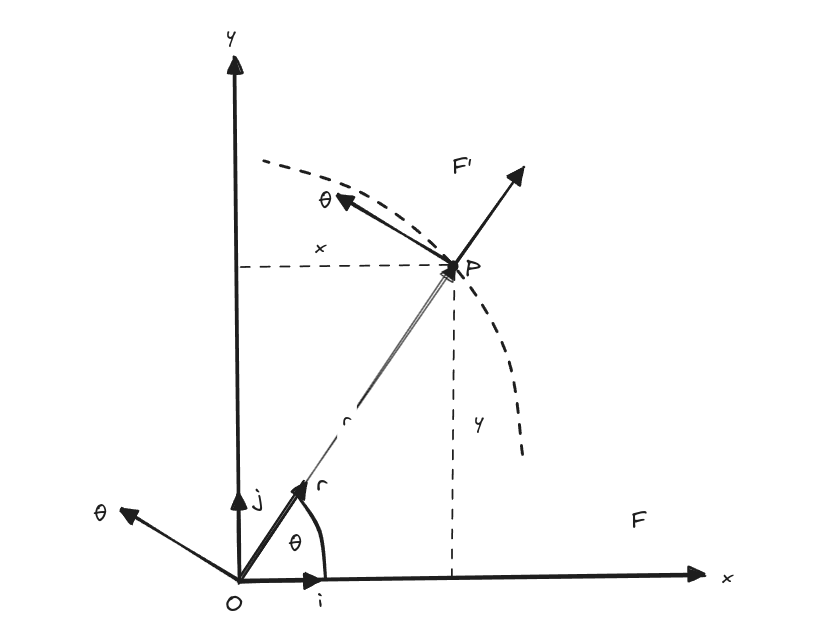
\includegraphics[scale=0.4]{ch17-1.png}
    \end{center}
    Let us consider another reference frame $\mathcal{F}'$ with axes in the
    directions of the unit vectors $\hatr$ and $\hatth$ where the origin
    coincides with the reference frame $\mathcal{F}$.
    The particle $P$ seen from $\mathcal{F}'$ has a position vector given 
    by $\bm{r}' = r \hatr$ where $\hatr$ is constant in this reference frame,
    so the velocity and acceleration of $P$ from this reference frame
    are $\bm{v}' = \dot r\hatr$ and $\bm{a}' = \ddot r\hatr$.
    So using the Velocity transformation formula we have that
    \begin{align*}
        \bm{v} &= \bm{V} + \bm\Omega \times \bm{r}' + \bm{v}'\\
            &= \dot\theta\hatn \times r \hatr + \dot r\hatr\\
            &= \dot\theta r \hatth + \dot r\hatr
    \end{align*}
    We used that $\bm\Omega = \dot\theta \hatn$ where $\hatn$ points in the
    normal direction to the plane also we used that $\bm r' = r \hatr$.

    In the same way, using the Acceleration transformation formula we have that
    \begin{align*}
        \bm{a} &= \bm{A} + \bm\dot\Omega \times \bm{r}' + 2\bm\Omega \times \bm v'
        + \bm\Omega \times (\bm\Omega \times \bm r') + \bm a'\\
        &= (\ddot\theta \hatn \times r\hatr)
        + (2\dot\theta \hatn \times \dot r \hatr)
        + (\dot\theta \hatn \times (\dot\theta \hatn \times r\hatr))
        + \ddot r\hatr\\
        &= \ddot\theta r \hatth + 2\dot\theta\dot r \hatth
        + \dot\theta \hatn \times (\dot\theta r\hatth) + \ddot r\hatr\\
        &= \ddot\theta r \hatth + 2\dot\theta\dot r \hatth
        - \dot\theta^2 r\hatr + \ddot r\hatr\\
        &= (r\ddot\theta + 2\dot r\dot\theta)\hatth
        +(\ddot r - r\dot\theta^2)\hatr
    \end{align*}
\end{proof}
\cleardoublepage
\begin{proof}{\textbf{17.2}}
    Let us consider a moving rigid body as shown below
    \begin{center}
        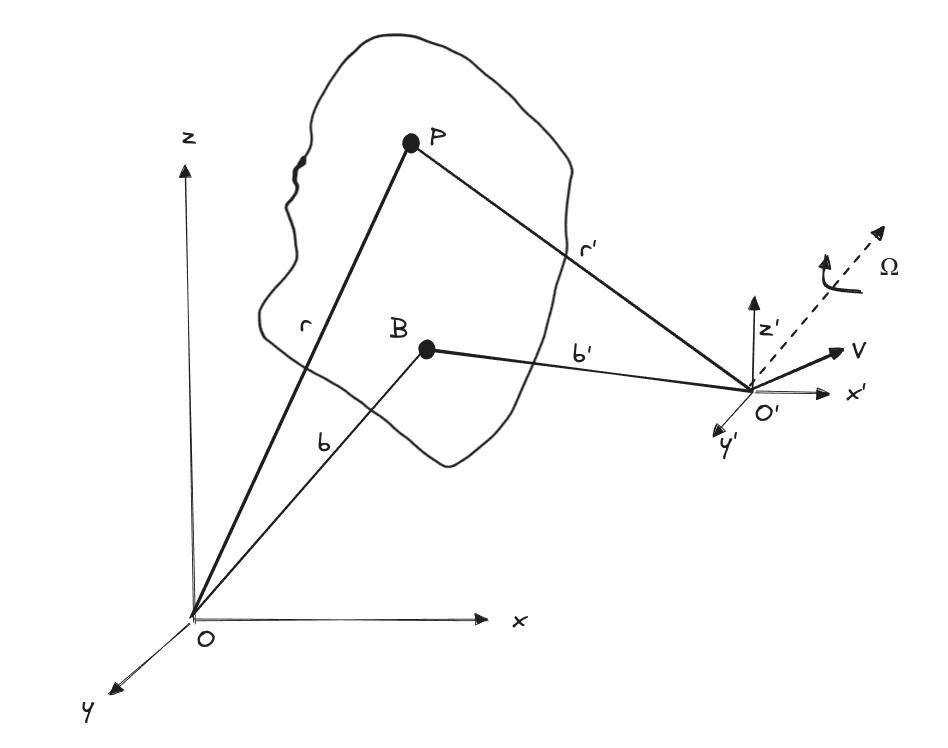
\includegraphics[scale=0.5]{ch17-2.png}
    \end{center}

    Then according to Chapter 16 the velocity of a particle $P$ of the rigid
    body from the reference frame $\mathcal{F} = \{O;x,y,z\}$ is given by
    \begin{align*}
        \bm{v} = \bm{v}^B + \bm{\omega}\times (\bm{r} - \bm{b})
    \end{align*}
    Where $\bm{r}$ and $\bm{b}$ are the position vectors of particle $P$ and
    $B$ respectively and $\bm{v}^B$ is the velocity of particle $B$.

    Now let us take another reference frame $\mathcal{F'} = \{O';x',y',z'\}$
    which has translational velocity $\bm{V}$ and angular velocity $\bm{\Omega}$
    with respect to $\mathcal{F}$ then the velocity of the particle $P$
    in this reference frame is given by
    \begin{align*}
        \bm{v}' = \bm{v}'^B + \bm{\omega}'\times (\bm{r}' - \bm{b}')
    \end{align*}
    Where $\bm{r}'$ and $\bm{b}'$ are the position vectors of particle $P$ and
    $B$ respectively in this reference frame and $\bm{v}'^B$ is the velocity
    of particle $B$ in this reference frame.
    On the other hand, using the velocity transformation formula we have that
    \begin{align*}
        \bm{v} &= \bm{V} + \bm{\Omega}\times \bm{r}' + \bm{v}'\\
        \bm{v} &= \bm{V} + \bm{\Omega}\times \bm{r}' + \bm{v}'^B
        + \bm{\omega}'\times (\bm{r}' - \bm{b}')\\
        \bm{v} &= \bm{V} + \bm{v}'^B + \bm{\Omega}\times \bm{r}'
        + \bm{\omega}'\times (\bm{r}' - \bm{b}')
        + \bm{\Omega}\times \bm{b}' - \bm{\Omega}\times \bm{b}'\\
        \bm{v} &= \bm{V} + \bm{\Omega}\times \bm{b}' + \bm{v}'^B
        + (\bm{\Omega} + \bm{\omega}')\times (\bm{r}' - \bm{b}')\\
        \bm{v} &= \bm{v}^B +
        (\bm{\Omega} + \bm{\omega}')\times (\bm{r} - \bm{b})\\
    \end{align*}
    Where we used that $\bm{v}^B = \bm{V} + \bm{\Omega}\times \bm{b}' + \bm{v}'^B$
    and that $\bm{r} - \bm{b} = \bm{r}' - \bm{b}'$

    Finally, we know that
    $\bm{v} = \bm{v}^B + \bm{\omega}\times (\bm{r} - \bm{b})$
    then by comparing these equations, we have that
    \begin{align*}
        \bm{\omega} = \bm{\Omega} + \bm{\omega}'
    \end{align*}
\end{proof}
\cleardoublepage
\begin{proof}{\textbf{17.4}}
    Let us consider the following system
    \begin{center}
        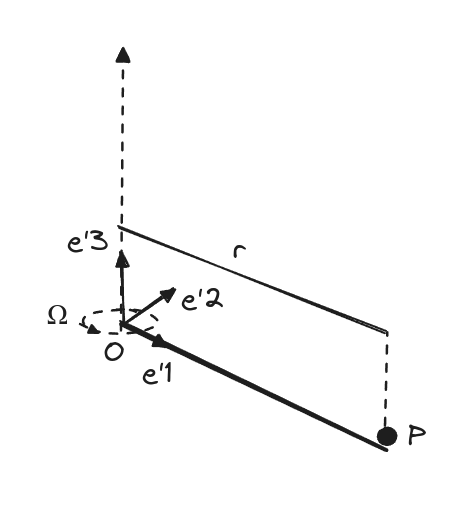
\includegraphics[scale=0.5]{ch17-4.png}
    \end{center}
    Let $\mathcal{F} = \{O; \bm e_1,\bm e_2,\bm e_3\}$ be an inertial reference
    frame and let  $\mathcal{F}' = \{O'; \bm e'_1,\bm e'_2,\bm e'_3\}$
    be a reference frame rotating with an angular velocity $\Omega$ with 
    respect to $\mathcal{F}$. Both reference frames share the same point as
    the origin.
    
    We see that $\mathcal{F}'$ has zero translational velocity and
    constant angular velocity $\bm\Omega =\Omega \bm e'_3$ relative to
    $\mathcal{F}$. Hence $\bm A = 0$ and $\bm{\dot\Omega} = 0$.

    From frame $\mathcal{F}'$ the particle is moving towards $O$ in a 
    rectilinear path so $\bm r' = r \bm e'_1$, $\bm{v}' = \dot{r} \bm{e}'_1$
    and $\bm{a}' = \ddot{r} \bm{e}'_1$.
    Then using the transformed equation of motion we have that
    \begin{align*}
        m[2\bm\Omega\times\bm{v}' + \bm\Omega\times(\bm\Omega\times \bm{r}')
        + \bm{a}'] &= \bm{F}\\
        2m\Omega \dot{r}\bm e'_2 - m\Omega^2 r\bm e'_1 + m \ddot{r} \bm{e}'_1
        &= -mg\bm e'_3 + N_1\bm e'_3 + N_2\bm e'_2
    \end{align*}
    Where $N_1, N_2$ are the normal forces applied to the particle by the wire
    Therefore the equation for the $\bm e'_1$ component is
    \begin{align*}
        m \ddot{r} - m\Omega^2 r &= 0\\
        \ddot{r} - \Omega^2 r &= 0
    \end{align*}
    We know that the solution to this differential equation is
    \begin{align*}
        r = C_1 e^{\Omega t} + C_2 e^{-\Omega t}
    \end{align*}
    Where $C_1$ and $C_2$ are constants. We know that the particle starts at
    rest at a distance $a$ from $O$. 
    But also we have that $\dot{r} = \Omega(C_1 e^{\Omega t} - C_2 e^{-\Omega t})$ 
    which implies, applying the initial conditions, that
    \begin{align*}
        0 &= C_1 - C_2\\ 
        C_1 &= C_2
    \end{align*}
    Also, applying the initial conditions to the $r$ equation we get that
    \begin{align*}
        a = C_1 + C_2 = 2C_1
    \end{align*}
    Therefore replacing $C_1$ in the equation we get that
    \begin{align*}
        r &= \frac{a}{2}e^{\Omega t} + \frac{a}{2} e^{-\Omega t}\\
            &= a\bigg(\frac{e^{\Omega t} + e^{-\Omega t}}{2}\bigg)\\
            &= a\cosh(\Omega t)
    \end{align*}
\end{proof}
\begin{proof}{\textbf{17.5}}
    Let $\mathcal{F}$ be a fixed reference frame and let $\mathcal{F}'$ be a
    rotating reference frame with respect to some axis that passes through
    the origin $O$ with an angular velocity $\bm\Omega$ then in this reference
    frame the equation of motion is given by
    \begin{align*}
        m[\bm{\dot\Omega} \times \bm{r}' + 2\bm\Omega \times \bm v'
        + \bm\Omega \times (\bm\Omega \times \bm r') + \bm a'] =
        \bigg(\frac{eB}{c}\bigg)
        ((\bm{\Omega}\times \bm{r}' + \bm{v}')\times \bm{k}) + \bm{F(r)}
    \end{align*}
    Since we want to remove the term $(eB/c)\bm{v}\times \bm{k}$ of the
    equation of motion in the reference frame $\mathcal{F}'$ we need
    to give some value to $\bm\Omega$ such that $\bm{v}' \times \bm{k}$
    cancels out and $(\bm\Omega\times \bm{r}') \times \bm{k} = 0$.
    So if we set $\bm\Omega$ as
    \begin{align*}
        \bm\Omega = -\bigg(\frac{eB}{2mc}\bigg)\bm{k}
    \end{align*}
    We get that
    \begin{align*}
        m[\bm{\dot\Omega} \times \bm{r}'
        &+ \bm\Omega \times (\bm\Omega \times \bm r') + \bm a'] 
        -\bigg(\frac{eB}{c}\bigg)\bm{k} \times \bm v' =\\
        & = \bigg(\frac{eB}{c}\bigg)
        \bigg(-\bigg(\frac{eB}{2mc}\bigg)\bm{k}\times \bm{r}'\bigg)\times \bm{k}
        + \bigg(\frac{eB}{c}\bigg)(\bm{v}'\times \bm{k}) + \bm{F(r)}
    \end{align*}
    Hence
    \begin{align*}
        m[\bm{\dot\Omega} \times \bm{r}'
        + \bm\Omega \times (\bm\Omega \times \bm r') + \bm a'] 
        = \bm{F(r)}
    \end{align*}
    Where we used that $(-\bm{k} \times \bm{r})\times \bm{k} = 0$ and that
    $-\bm{k} \times \bm{v}' = \bm{v}' \times \bm{k}$.

    For the last part, let $\bm{F(r)} = -m\omega_0^2\bm{r}$
    then since $\mathcal{F}'$ share the origin with $\mathcal{F}$ then
    $$\bm{F(r)} = -m\omega_0^2\bm{r} = -m\omega_0^2\bm{r}' = \bm{F(r')}$$
    and since
    $\bm{\Omega} = -K\bm{k}$ for some constant $K$
    then $\bm{\dot\Omega} = 0$ and hence the equation of motion is given by
    \begin{align*}
        m\bm{a}' &= -m(-K\bm{k} \times (-K\bm{k} \times \bm r'))
        - m\omega_0^2\bm{r}'\\
        \bm{a}' &= -K^2(\bm{k} \times (\bm{k} \times \bm r'))
        - \omega_0^2\bm{r}'\\
        \bm{a}' &= -K^2(r_k\bm{k} - \bm{r}')
        - \omega_0^2\bm{r}'
    \end{align*}
    Where $r_k$ is the component of $r$ in the $k$ direction. Though we can
    always choose the origin to be somewhere where $r_k = 0$ since the motion
    is planar then
    \begin{align*}
        \derivative{\bm{v}'}{t} &= (K^2 - \omega_0^2)\bm{r}'
    \end{align*}
    Or 
    \begin{align*}
        \derivative[2]{\bm{r}'}{t} + (\omega_0^2- K^2)\bm{r}' = 0
    \end{align*}
    Which is a system of Simple Harmonic Motion equations and hence the
    angular frequencies of these SHM are
    \begin{align*}
        \pm\sqrt{\omega_0^2- \bigg(\frac{eB}{2mc}\bigg)^2}
    \end{align*}
\end{proof}
\cleardoublepage
\begin{proof}{\textbf{17.6}}
    Let us consider the bullet is fired from a point on earth of co-latitude
    $\beta$ with a velocity $u$ in the $\bm{k}$ direction. 
    \begin{center}
        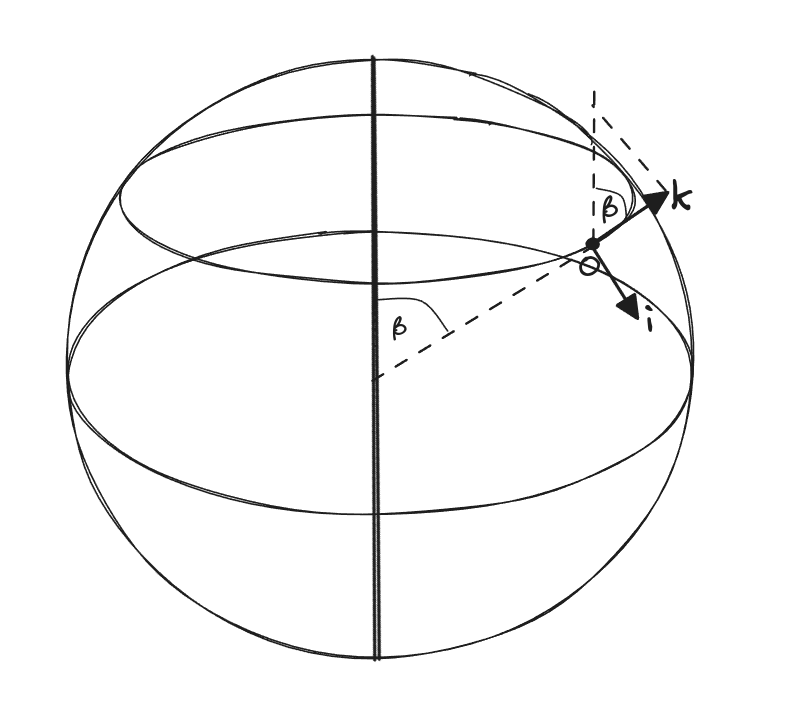
\includegraphics[scale=0.4]{ch17-6.png}
    \end{center}
    By using the projectile equation for a rotating Earth we have that
    \begin{align*}
        \derivative{\bm v}{t} + 2\bm{\Omega}\times \bm v = -g\bm{k}
    \end{align*}
    By integrating the equation with respect to $t$ we get that
    \begin{align*}
        \derivative{\bm r}{t} + 2\bm{\Omega}\times \bm{r} = -gt\bm{k}  + \bm{C}
    \end{align*}
    Where $\bm{C}$ is a constant of integration, and since
    $d\bm{r}/dt = u\bm{k}$ and $\bm{r} = 0$ when $t = 0$ we have that
    $\bm{C} = u\bm{k}$ therefore
    \begin{align*}
        \derivative{\bm r}{t} + 2\bm{\Omega}\times \bm{r} = (u - gt)\bm{k}
    \end{align*}
    Since we expect the effect of the Earth's rotation to be a small correction,
    we will solve this equation approximately by an iterative method.
    On integrating the equation with respect to $t$ and using the 
    initial conditions, we find that the unknown displacement $\bm{r}(t)$
    satisfies the following equation
    \begin{align*}
        \bm r(t)
        &= (ut - \frac{1}{2}gt^2)\bm{k}
        - 2\bm{\Omega}\times \int_0^t \bm{r}(t')~dt'
    \end{align*}
    We now solve this equation approximately by iteration. The zeroth order
    approximation $\bm{r}^{(0)}$ corresponds to the case $\Omega = 0$. Thus
    the zeroth order approximation is
    \begin{align*}
        \bm r^{(0)} &= (ut - \frac{1}{2}gt^2)\bm{k}
    \end{align*}
    which is just the elementary solution for vertical motion under uniform
    gravity. The first order approximation $\bm{r}^{(1)}$ is now obtained
    by substituting the zeroth order approximation into the integral term in
    the equation as follows
    \begin{align*}
        \bm r^{(1)}
        &= (ut - \frac{1}{2}gt^2)\bm{k}
        - 2\bm{\Omega}\times \int_0^t (ut' - \frac{1}{2}gt'^2)\bm{k}~dt'\\
        &= (ut - \frac{1}{2}gt^2)\bm{k}
        - \bigg(
            ut^2 - \frac{1}{3}gt^3
        \bigg)(\bm{\Omega}\times\bm{k})
    \end{align*}
    We know the Earth's angular velocity $\bm{\Omega}$ is
    \begin{align*}
        \bm{\Omega} = \Omega(-\sin\beta\bm{i} + \cos\beta \bm{k})
    \end{align*}
    where $\beta$ is the co-latitude of the origin $O$.
    It follows that $\bm{\Omega}\times\bm{k} = \Omega\sin\beta \bm{j}$
    and so the first order approximation for the displacement $\bm{r}(t)$
    is given by
    \begin{align*}
        \bm r^{(1)}
        &= (ut - \frac{1}{2}gt^2)\bm{k}
        - \bigg(ut^2 - \frac{1}{3}gt^3\bigg)\Omega\sin\beta \bm{j}
    \end{align*}
    We see that the bullet will not travel through the apparent vertical,
    but will be displaced in the positive $\bm{j}$-direction. We want to 
    determine this displacement in terms of the constants we have, so we need
    the travel time of the bullet.

    When the bullet arrives at the highest point the velocity will be $0$ so
    if we derivate the zeroth order approximation and we say that
    $d\bm{r}/dt = 0$ we get the time it takes for the bullet to 
    the highest point correct to the zeroth-order approximation as follows
    \begin{align*}
        0 &= u - gt\\
        t &= \frac{u}{g}
    \end{align*}
    If we assume this time is also correct for the first-order approximation
    and we multiply it by 2 to take into account the downward travel time we
    get that the displacement in the positive $\bm{j}$-direction is
    \begin{align*}
        \bigg(4\frac{u^3}{g^2} - \frac{8}{3}g\frac{u^3}{g^3}\bigg)
        \Omega\sin\beta =
        \frac{u^3}{g^2}\bigg(4 - \frac{8}{3}\bigg)\Omega\sin\beta =
        \frac{4\Omega u^3\sin\beta}{3g^2}
    \end{align*}
\end{proof}
\cleardoublepage
\begin{proof}{\textbf{17.7}}
    Let us consider the artillery shell is fired from a point on earth of
    co-latitude $\beta$ with a velocity $u$ in the
    $\sin\alpha\bm{k} + \cos\alpha \bm{i}$ direction.
    By using the projectile equation for a rotating Earth we have that
    \begin{align*}
        \derivative{\bm v}{t} + 2\bm{\Omega}\times \bm v = -g\bm{k}
    \end{align*}
    By integrating the equation with respect to $t$ we get that
    \begin{align*}
        \derivative{\bm r}{t} + 2\bm{\Omega}\times \bm{r} = -gt\bm{k}  + \bm{C}
    \end{align*}
    Where $\bm{C}$ is a constant of integration, and since
    $d\bm{r}/dt = u(\sin\alpha\bm{k} + \cos\alpha \bm{i})$ and $\bm{r} = 0$ when $t = 0$ we have that
    $\bm{C} = u(\sin\alpha\bm{k} + \cos\alpha \bm{i})$ therefore
    \begin{align*}
        \derivative{\bm r}{t} + 2\bm{\Omega}\times \bm{r}
        = (u\sin\alpha - gt)\bm{k} + u\cos\alpha \bm{i}
    \end{align*}
    Since we expect the effect of the Earth's rotation to be a small correction,
    we will solve this equation approximately by an iterative method.
    On integrating the equation with respect to $t$ and using the 
    initial conditions, we find that the unknown displacement $\bm{r}(t)$
    satisfies the following equation
    \begin{align*}
        \bm r(t)
        &= (ut\sin\alpha - \frac{1}{2}gt^2)\bm{k} + ut\cos\alpha \bm{i}  
        - 2\bm{\Omega}\times \int_0^t \bm{r}(t')~dt'
    \end{align*}
    We now solve this equation approximately by iteration. The zeroth order
    approximation $\bm{r}^{(0)}$ corresponds to the case $\Omega = 0$. Thus
    the zeroth order approximation is
    \begin{align*}
        \bm r^{(0)} &= (ut\sin\alpha - \frac{1}{2}gt^2)\bm{k} + ut\cos\alpha \bm{i}
    \end{align*}
    which is just the elementary solution for the parabolic motion under
    uniform gravity.
    The first order approximation $\bm{r}^{(1)}$ is now obtained
    by substituting the zeroth order approximation into the integral term in
    the equation as follows
    \begin{align*}
        \bm r^{(1)}
        &= (ut\sin\alpha - \frac{1}{2}gt^2)\bm{k} + ut\cos\alpha \bm{i} \\
        &\quad- 2\bm{\Omega}\times \int_0^t
        (ut'\sin\alpha - \frac{1}{2}gt'^2)\bm{k} + ut'\cos\alpha \bm{i}~dt'\\
        &= (ut\sin\alpha - \frac{1}{2}gt^2)\bm{k} + ut\cos\alpha \bm{i}\\
        &\quad- 2\bm{\Omega}\times
        \bigg[\bigg(\frac{1}{2}ut^2\sin\alpha - \frac{1}{6}gt^3\bigg)\bm{k}
        + \frac{1}{2}ut^2\cos\alpha \bm{i}\bigg]\\
        &= (ut\sin\alpha - \frac{1}{2}gt^2)\bm{k} + ut\cos\alpha \bm{i}\\
        &\quad- \bm{\Omega}\times
        \bigg[\bigg(ut^2\sin\alpha - \frac{1}{3}gt^3\bigg)\bm{k}
        + ut^2\cos\alpha \bm{i}\bigg]
    \end{align*}
    We know the Earth's angular velocity $\bm{\Omega}$ is
    \begin{align*}
        \bm{\Omega} = \Omega(-\sin\beta\bm{i} + \cos\beta \bm{k})
    \end{align*}
    where $\beta$ is the co-latitude of the origin $O$.
    It follows that $\bm{\Omega}\times\bm{k} = \Omega\sin\beta \bm{j}$
    and $\bm{\Omega}\times\bm{i} = \Omega\cos\beta \bm{j}$
    and so the first order approximation for the displacement $\bm{r}(t)$
    is given by
    \begin{align*}
        \bm r^{(1)}
        &= (ut\sin\alpha - \frac{1}{2}gt^2)\bm{k} + ut\cos\alpha \bm{i}\\
        &\quad-\bigg[\bigg(ut^2\sin\alpha - \frac{1}{3}gt^3\bigg)
        \Omega\sin\beta\bm{j}
        + ut^2\cos\alpha \Omega\cos\beta\bm{j}\bigg]\\
        &= (ut\sin\alpha - \frac{1}{2}gt^2)\bm{k} + ut\cos\alpha \bm{i}\\
        &\quad-\bigg[ut^2\Omega\bigg(\sin\alpha\sin\beta
        + \cos\alpha\cos\beta\bigg)
        - \frac{1}{3}gt^3\Omega\sin\beta
        \bigg]\bm{j}
    \end{align*}
    We see that the artillery shell will not travel through the apparent
    parabolic path, but will be displaced in the positive $\bm{j}$-direction.
    We want to determine this displacement in terms of the constants we have,
    so we need the travel time of the shell.

    When the artillery shell arrives at the highest point the velocity will be
    $0$ so if we derivate the zeroth order approximation and we say that
    $d\bm{r}/dt = 0$ we get the time it takes for the shell to 
    the highest point correct to the zeroth-order approximation.
    In what follows we only consider the $\bm{k}$ direction of the velocity
    since the $\bm{i}$ direction does not give us any information 
    \begin{align*}
        0 &= u\sin\alpha - gt\\
        t &= \frac{u\sin\alpha}{g}
    \end{align*}
    If we assume this time is also correct for the first-order approximation
    and we multiply it by 2 to take into account the downward travel time we
    get that the displacement in the positive $\bm{j}$-direction is
    \begin{align*}
        &
        u\frac{4u^2\sin^2\alpha}{g^2}\Omega\bigg(\sin\alpha\sin\beta
        + \cos\alpha\cos\beta\bigg)
        -\frac{1}{3}g\frac{8u^3\sin^3\alpha}{g^3}\Omega\sin\beta =\\
        &\qquad= \frac{4u^3\Omega\sin^2\alpha}{g^2}\bigg(\sin\alpha\sin\beta
        + \cos\alpha\cos\beta\bigg)
        - \frac{8u^3\Omega\sin^2\alpha}{3g^2}\sin\alpha\sin\beta\\
        &\qquad= \frac{4u^3\Omega\sin^2\alpha}{3g^2}
        (3(\sin\alpha\sin\beta + \cos\alpha\cos\beta) - 2\sin\alpha\sin\beta)\\
        &\qquad= \frac{4u^3\Omega\sin^2\alpha}{3g^2}
        (\sin\alpha\sin\beta + 3\cos\alpha\cos\beta)
    \end{align*}
\end{proof}
\cleardoublepage
\begin{proof}{\textbf{17.8}}
    Let us consider the artillery shell is fired from a point on earth of
    co-latitude $\beta$ with a velocity $u$ in the
    $\sin\alpha\bm{k} + \cos\alpha \bm{j}$ direction.
    By using the projectile equation for a rotating Earth we have that
    \begin{align*}
        \derivative{\bm v}{t} + 2\bm{\Omega}\times \bm v = -g\bm{k}
    \end{align*}
    By integrating the equation with respect to $t$ we get that
    \begin{align*}
        \derivative{\bm r}{t} + 2\bm{\Omega}\times \bm{r} = -gt\bm{k}  + \bm{C}
    \end{align*}
    Where $\bm{C}$ is a constant of integration, and since
    $d\bm{r}/dt = u(\sin\alpha\bm{k} + \cos\alpha \bm{j})$ and $\bm{r} = 0$ when $t = 0$ we have that
    $\bm{C} = u(\sin\alpha\bm{k} + \cos\alpha \bm{j})$ therefore
    \begin{align*}
        \derivative{\bm r}{t} + 2\bm{\Omega}\times \bm{r}
        = (u\sin\alpha - gt)\bm{k} + u\cos\alpha \bm{j}
    \end{align*}
    Since we expect the effect of the Earth's rotation to be a small correction,
    we will solve this equation approximately by an iterative method.
    On integrating the equation with respect to $t$ and using the 
    initial conditions, we find that the unknown displacement $\bm{r}(t)$
    satisfies the following equation
    \begin{align*}
        \bm r(t)
        &= (ut\sin\alpha - \frac{1}{2}gt^2)\bm{k} + ut\cos\alpha \bm{j}  
        - 2\bm{\Omega}\times \int_0^t \bm{r}(t')~dt'
    \end{align*}
    We now solve this equation approximately by iteration. The zeroth order
    approximation $\bm{r}^{(0)}$ corresponds to the case $\Omega = 0$. Thus
    the zeroth order approximation is
    \begin{align*}
        \bm r^{(0)} &= (ut\sin\alpha - \frac{1}{2}gt^2)\bm{k} + ut\cos\alpha \bm{j}
    \end{align*}
    which is just the elementary solution for the parabolic motion under
    uniform gravity.
    The first order approximation $\bm{r}^{(1)}$ is now obtained
    by substituting the zeroth order approximation into the integral term in
    the equation as follows
    \begin{align*}
        \bm r^{(1)}
        &= (ut\sin\alpha - \frac{1}{2}gt^2)\bm{k} + ut\cos\alpha \bm{j} \\
        &\quad- 2\bm{\Omega}\times \int_0^t
        (ut'\sin\alpha - \frac{1}{2}gt'^2)\bm{k} + ut'\cos\alpha \bm{j}~dt'\\
        &= (ut\sin\alpha - \frac{1}{2}gt^2)\bm{k} + ut\cos\alpha \bm{j}\\
        &\quad- 2\bm{\Omega}\times
        \bigg[\bigg(\frac{1}{2}ut^2\sin\alpha - \frac{1}{6}gt^3\bigg)\bm{k}
        + \frac{1}{2}ut^2\cos\alpha \bm{j}\bigg]\\
        &= (ut\sin\alpha - \frac{1}{2}gt^2)\bm{k} + ut\cos\alpha \bm{j}\\
        &\quad- \bm{\Omega}\times
        \bigg[\bigg(ut^2\sin\alpha - \frac{1}{3}gt^3\bigg)\bm{k}
        + ut^2\cos\alpha \bm{j}\bigg]
    \end{align*}
    We know the Earth's angular velocity $\bm{\Omega}$ is
    \begin{align*}
        \bm{\Omega} = \Omega(-\sin\beta\bm{i} + \cos\beta \bm{k})
    \end{align*}
    where $\beta$ is the co-latitude of the origin $O$.
    It follows that $\bm{\Omega}\times\bm{k} = \Omega\sin\beta \bm{j}$
    and $\bm{\Omega}\times\bm{j} = \Omega(-\sin\beta\bm{k} - \cos\beta \bm{i})$
    and so the first order approximation for the displacement $\bm{r}(t)$
    is given by
    \begin{align*}
        \bm r^{(1)}
        &= (ut\sin\alpha - \frac{1}{2}gt^2)\bm{k} + ut\cos\alpha \bm{j}\\
        &\quad-\bigg[
            \bigg(ut^2\sin\alpha - \frac{1}{3}gt^3\bigg)\Omega\sin\beta\bm{j}
            + ut^2\cos\alpha \Omega(-\sin\beta\bm{k} - \cos\beta \bm{i})
        \bigg]\\
        &= \bigg(
            ut\sin\alpha - \frac{1}{2}gt^2
            + ut^2\Omega\cos\alpha\sin\beta
        \bigg)\bm{k}\\
        &\quad + \bigg[ut\cos\alpha - \bigg(
            ut^2\sin\alpha - \frac{1}{3}gt^3
        \bigg)\Omega\sin\beta\bigg] \bm{j}\\
        &\quad + (ut^2\Omega\cos\alpha \cos\beta)\bm{i}
    \end{align*}
    We see that the artillery shell will not travel through the apparent
    parabolic path on the $yz$-plane, but will be displaced to the
    $\bm{i}$-direction too.
    We want to determine this displacement in terms of the constants we have,
    so we need the travel time of the shell.

    When the artillery shell arrives at the highest point the velocity will be
    $0$ so if we derivate the zeroth order approximation and we say that
    $d\bm{r}/dt = 0$ we get the time it takes for the shell to 
    the highest point correct to the zeroth-order approximation.
    In what follows we only consider the $\bm{k}$ direction of the velocity
    since the $\bm{j}$ direction does not give us any information 
    \begin{align*}
        0 &= u\sin\alpha - gt\\
        t &= \frac{u\sin\alpha}{g}
    \end{align*}
    If we assume this time is also correct for the first-order approximation
    and we multiply it by 2 to take into account the downward travel time we
    get that the displacement in the $\bm{i}$ direction is
    \begin{align*}
        u\frac{4u^2\sin^2\alpha}{g^2}\Omega(\cos\alpha\cos\beta) &=
        \frac{4u^3\Omega\sin^2\alpha}{g^2}(\cos\alpha\cos\beta)
    \end{align*}
    Now we want to compute the increased east range 
    but for this we need the travel time correct to the first-order so
    we derivate the $\bm{k}$ component of $\bm{r}^{(1)}$ and we make it equal
    to 0 to get the travel time $t$ to the highest point as shown below
    \begin{align*}
        u\sin\alpha - gt + 2ut\Omega\cos\alpha\sin\beta &= 0\\
        t(g - 2u\Omega\cos\alpha\sin\beta) &= u\sin\alpha\\
        t &= \frac{u\sin\alpha}{g - 2u\Omega\cos\alpha\sin\beta}
    \end{align*}
    We can apply also the binomial approximation since
    $2u\Omega\cos\alpha\sin\beta/g$ is small then
    \begin{align*}
        t &= \frac{u\sin\alpha}{g}
        \bigg(1 - \frac{2u\Omega\cos\alpha\sin\beta}{g}\bigg)^{-1}
        \approx \frac{u\sin\alpha}{g}
        \bigg(1 + \frac{2u\Omega}{g}\cos\alpha\sin\beta\bigg)
    \end{align*}
    Now given that the eastern displacement has terms involving $t$, $t^2$ and
    $t^3$ we replace the zeroth-approximation for $t$ on $t^2$ and $t^3$ since
    they are small and the first-approximation in $t$ as follows
    \begin{align*}
        &u\frac{2u\sin\alpha}{g}
        \bigg(1 + \frac{2u\Omega}{g}\cos\alpha\sin\beta\bigg)
        \cos\alpha
        - \bigg(
            u\frac{4u^2\sin^2\alpha}{g^2}\sin\alpha
            - \frac{1}{3}g\frac{8u^3\sin^3\alpha}{g^3}
        \bigg)\Omega\sin\beta =\\
        &= \frac{2u^2\sin\alpha}{g}
        \bigg(1 + \frac{2u\Omega}{g}\cos\alpha\sin\beta\bigg)
        \cos\alpha
        - \frac{4u^3\sin^3\alpha}{3g^2}\Omega\sin\beta =\\
        &= \frac{4\Omega u^3}{3g^2}\sin\alpha\sin\beta\bigg(
            \frac{3g}{2\Omega u}\frac{\cos\alpha}{\sin\beta}
            + 3\cos^2\alpha - \sin^2\alpha\bigg)=\\
        &= \frac{4\Omega u^3}{3g^2}\sin\alpha\sin\beta\bigg(
            \frac{3g}{2\Omega u}\frac{\cos\alpha}{\sin\beta}
            + 3 - 4\sin^2\alpha\bigg)
    \end{align*}
    Therefore we see that the easterly range is increased by
    \begin{align*}
        \frac{4\Omega u^3}{3g^2}\sin\alpha\sin\beta
        (3 - 4\sin^2\alpha)
    \end{align*} 
\end{proof}
\cleardoublepage
\begin{proof}{\textbf{17.9}}
    Let us consider the system described below
    \begin{center}
        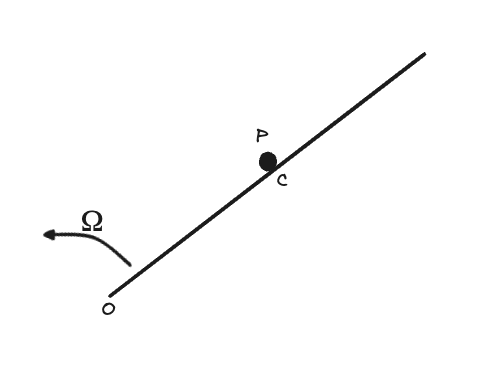
\includegraphics[scale=0.4]{ch17-9.png}
    \end{center}
    We will view the motion of the particle from a reference frame with origin
    $O$ in which the wire is at rest.
    This frame has a fixed origin and constant angular velocity.
    
    Let $r$ be the distance $OC$ then in the rotating frame, the motion of the
    particle is rectilinear and its apparent kinetic energy is therefore 
    given by $T = 1/2m\dot r^2$.

    Now we find the apparent potential energy. There are no specified external
    forces, but there is the constraint force exerted on the particle by the
    wire, which, since the wire is smooth, acts perpendicular to the wire.
    In an inertial frame, this constraint force does work, but, in the frame
    rotating with the wire, the particle simply moves along the stationary
    wire. The apparent rate of working of the constraint force is therefore
    zero. The system is therefore apparently conservative with potential energy
    $V=0$.

    The transformed energy equation is therefore
    \begin{align*}
        \frac{1}{2}m\dot r^2 - \frac{1}{2}(mr^2)\Omega^2 = E 
    \end{align*}
    Where $mr^2$ is the moment of inertia of the particle about the vertical
    axis through $O$, and $\Omega$ is the angular speed of the wire.

    So with the initial conditions $r = a$ and $\dot r = 0$ when $t=0$ we get
    that
    \begin{align*}
        E = - \frac{1}{2}(ma^2)\Omega^2
    \end{align*}
    Therefore the transformed energy equation is given by
    \begin{align*}
        \dot r^2 - r^2\Omega^2 &= - a^2\Omega^2\\
        \dot r &= \Omega\sqrt{r^2 - a^2}
    \end{align*}
    By integration we get that the equation of motion for the particle is 
    \begin{align*}
        \int_0^r \frac{dr}{\sqrt{r^2 - a^2}} &= \Omega \int_0^t dt
    \end{align*}
    Let $r = a \cosh(u)$ then $dr = a\sinh(u) du$ hence
    \begin{align*}
        \Omega t &= \int_0^u \frac{a\sinh(u) du}{\sqrt{a^2\cosh^2(u) - a^2}}\\
        &= \int_0^u \frac{\sinh(u) du}{\sqrt{\cosh^2(u) - 1}}\\
        &= \int_0^u \frac{\sinh(u) du}{\sqrt{\sinh^2(u)}}\\
        &= u
    \end{align*}
    But $u = \cosh^{-1}(r/a)$ hence
    \begin{align*}
        \cosh^{-1}\bigg(\frac{r}{a}\bigg) &= \Omega t\\
        r &= a\cosh(\Omega t)
    \end{align*}
    Which is the same result we got for Problem 17.4.
\end{proof}
\cleardoublepage
\begin{proof}{\textbf{17.10}}
    Let us consider the system described below
    \begin{center}
        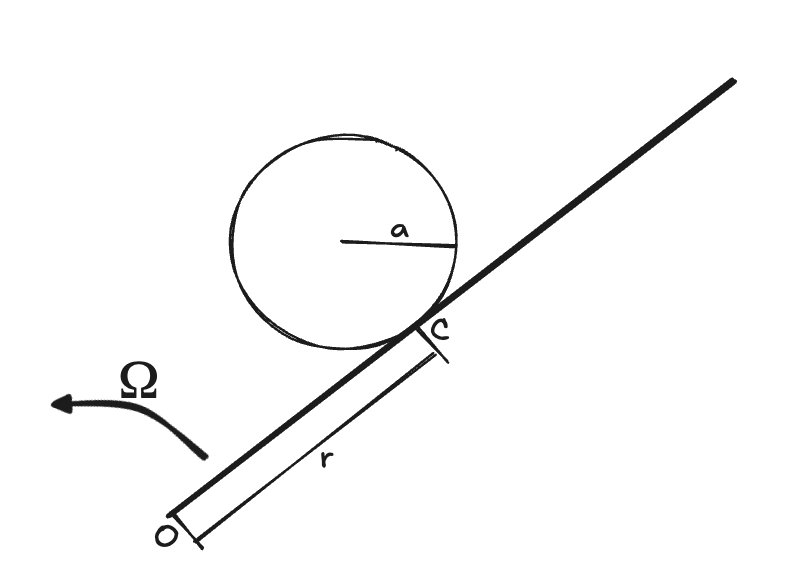
\includegraphics[scale=0.4]{ch17-10.png}
    \end{center}
    We will view the motion of the disk from a reference frame with origin
    $O$ in which the rod is at rest.
    This frame has a fixed origin and constant angular velocity.
    
    Let $r$ be the distance $OC$ then in the rotating frame, the
    disk is rolling and its apparent kinetic energy is therefore 
    given by
    $$T = \frac{1}{2}M\dot r^2
    + \frac{1}{2}\bigg(\frac{1}{2} M a^2\bigg)\bigg(\frac{\dot r}{a}\bigg)^2$$
    where $\dot r$ is the velocity of the disk's centre of mass.

    Now we find the apparent potential energy. There are no specified external
    forces, but there is the constraint force exerted on the disk by the
    rod, which acts perpendicular to the rod.
    In an inertial frame, this constraint force does work, but, in the frame
    rotating with the rod, the disk simply rolls along the stationary
    rod. The apparent rate of working of the constraint force is therefore
    zero. The system is therefore apparently conservative with potential energy
    $V=0$.

    The transformed energy equation is therefore
    \begin{align*}
        \frac{3}{4}M\dot r^2
        - \frac{1}{2}\bigg(\frac{1}{2}Ma^2 + M(r^2 + a^2)\bigg)\Omega^2 = E 
    \end{align*}
    Here $\frac{1}{2}Ma^2 + M(r^2 + a^2)$ is the moment of inertia of the disk
    about the vertical axis through $O$ where we used the parallel axes theorem
    and that the distance from $O$ to the centre of mass of the disk is
    $\sqrt{r^2 + a^2}$. Also, $\Omega$ is the angular speed of the rod.

    So with the initial conditions $r = a$ and $\dot r = 0$ when $t=0$ we get
    that
    \begin{align*}
        E = - \frac{1}{2}\bigg(\frac{5}{2}Ma^2\bigg)\Omega^2
        = - \frac{5}{4}Ma^2\Omega^2
    \end{align*}
    Therefore the transformed energy equation is given by
    \begin{align*}
        \frac{3}{4}M\dot r^2
        - \frac{1}{2}\bigg(\frac{1}{2}Ma^2 + M(r^2 + a^2)\bigg)\Omega^2
        &= - \frac{5}{4}Ma^2\Omega^2\\
        \frac{3}{2}\dot r^2
        - \frac{1}{2}a^2\Omega^2 - (r^2 + a^2)\Omega^2
        &= - \frac{5}{2}a^2\Omega^2
    \end{align*}
    Hence
    \begin{align*}
        \dot r^2&= (r^2 + a^2)\Omega^2 - 2a^2\Omega^2\\
        \dot r &= \sqrt{\frac{2}{3}}\Omega\sqrt{(r^2 + a^2) - 2a^2}\\
        \dot r &= \sqrt{\frac{2}{3}}\Omega\sqrt{r^2 - a^2}
    \end{align*}
    By integration as we did in the previous problem we get the displacement
    of the disk as a function of time
    \begin{align*}
        r &= a\cosh\bigg(\sqrt{\frac{2}{3}}\Omega t\bigg)
    \end{align*}
\end{proof}
\cleardoublepage
\begin{proof}{\textbf{17.11}}
    Let us consider the system described below
    \begin{center}
        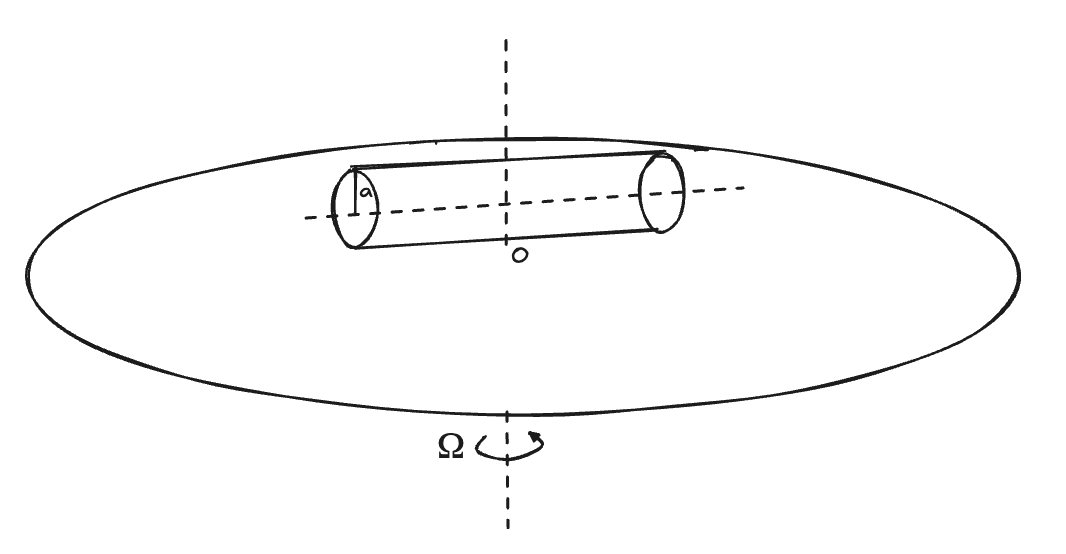
\includegraphics[scale=0.3]{ch17-11.png}
    \end{center}
    We will view the motion of the cylinder from a reference frame with origin
    $O$ in which the cylinder is at rest.
    This frame has a fixed origin and constant angular velocity $\Omega$.
    From this reference frame the cylinder is at rest before the disturbance
    and rolling after it.

    Let $x$ be the distance that the cylinder moves after the disturbance
    (by rolling)
    \begin{center}
        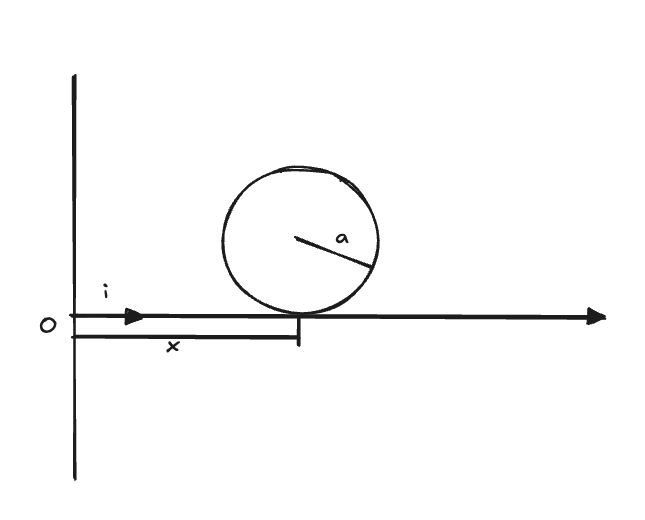
\includegraphics[scale=0.3]{ch17-11-1.png}
    \end{center}   
    Then the apparent kinetic energy is given by
    $$T = \frac{1}{2}M\dot x^2
    + \frac{1}{2}(M a^2)\bigg(\frac{\dot x}{a}\bigg)^2$$
    where $\dot x$ is the velocity of the cylinder's centre of mass and $Ma^2$
    is the moment of inertia of the cylinder.

    Now we find the apparent potential energy. There are no specified external
    forces, but there is the constraint force exerted on the cylinder by the
    turntable, which acts perpendicular to the cylinder.
    In an inertial frame, this constraint force does work, but, in the frame
    rotating with the turntable, the cylinder simply rolls along the stationary
    turntable. The apparent rate of working of the constraint force is therefore
    zero. The system is therefore apparently conservative with potential energy
    $V=0$.
    
    The transformed energy equation is therefore
    \begin{align*}
        M\dot x^2
        - \frac{1}{2}\bigg(\frac{1}{2}Ma^2 + M(x^2 + a^2)\bigg)\Omega^2 = E 
    \end{align*}
    Here $\frac{1}{2}Ma^2 + M(x^2 + a^2)$ is the moment of inertia
    of the cylinder about the vertical axis through $O$ where we used the
    parallel axes theorem and that the distance from $O$ to the centre of mass
    of the cylinder is $\sqrt{x^2 + a^2}$.
    Also, $\Omega$ is the angular speed of the turntable.

    So with the initial conditions $x = 0$ and $\dot x = 0$ when $t=0$ we get
    that
    \begin{align*}
        E = - \frac{3}{4}Ma^2\Omega^2
    \end{align*}
    Therefore the transformed energy equation is given by
    \begin{align*}
        M\dot x^2
        - \frac{1}{2}\bigg(\frac{1}{2}Ma^2 + M(x^2 + a^2)\bigg)\Omega^2
        &= - \frac{3}{4}Ma^2\Omega^2\\
        \dot x^2
        - \frac{1}{2}\bigg(\frac{1}{2}a^2 + (x^2 + a^2)\bigg)\Omega^2
        &= - \frac{3}{4}a^2\Omega^2\\
        \dot x^2 - \frac{1}{2}x^2\Omega^2 - \frac{3}{4}a^2\Omega^2
        &= - \frac{3}{4}a^2\Omega^2
    \end{align*}
    Hence the velocity of the cylinder is 
    \begin{align*}
        \dot x^2&= \frac{1}{2}x^2\Omega^2\\
        \dot x&= \frac{x\Omega}{\sqrt{2}}
    \end{align*}
    Considering the rotating reference frame with a constant angular velocity
    of $\bm\Omega = \Omega \bm{k}$ then the Second Law in a general
    non-inertial frame is 
    \begin{align*}
        M[
            2\bm\Omega\times\bm{\dot x}
            + \bm{\Omega}\times(\bm{\Omega}\times \bm{x}) + \bm{\ddot{x}}
        ] &= \bm{F}\\
        M\bigg[
            2\Omega\uvk \times \frac{x\Omega}{\sqrt{2}}\uvi
            + \Omega\uvk \times (\Omega\uvk \times x\bm{i})
            + \ddot x\uvi
        \bigg] &= -Mg\uvk + \bm{N}
    \end{align*}
    But also if we use that
    \begin{align*}
        \ddot x&= \frac{\dot x\Omega}{\sqrt{2}}
        = \frac{x\Omega^2}{2}
    \end{align*}
    We get that
    \begin{align*}
        M\bigg[
            2\Omega\uvk \times \frac{x\Omega}{\sqrt{2}}\uvi
            + \Omega\uvk \times (\Omega\uvk \times x\bm{i})
            + \frac{\Omega^2 x}{2}\uvi
        \bigg] &= -Mg\uvk + \bm{N}
    \end{align*}
    Where we set that $\uvi$ points in the direction of the motion and
    $\uvk$ points vertically upward. Also, $\bm{N}$ is the force that
    the turntable exerts on the cylinder. Therefore we get that
    \begin{align*}
        \bm{N} -Mg\uvk &= M\bigg[
            \frac{2x\Omega^2}{\sqrt{2}}\uvj
            -\Omega^2 x \uvi
            + \frac{\Omega^2 x}{2}\uvi
        \bigg]\\
        \bm{N} &= Mg\uvk + \sqrt{2}M\Omega^2x\uvj - \frac{1}{2}M\Omega^2 x\uvi
    \end{align*}
\end{proof}
\cleardoublepage
\begin{proof}{\textbf{17.12}}
    Let us see the rotating bucket of water from a reference frame which is
    rotating with the same angular velocity $\bm{\Omega} = \Omega\uvk$
    then the equation of hydrostatics in this frame is 
    \begin{align*}
        \rho\bm{\Omega} \times (\bm{\Omega} \times \bm{r}) &= -\rho g\hatz - \grad p\\
        \rho\Omega\hatz \times (\Omega\hatz \times \bm{r}) &= -\rho g\hatz - \grad p
    \end{align*}
    Where we used that $\bm{F} = -\rho g\hatz$. So in cylindrical coordinates
    we have that
    \begin{align*}
        \rho\Omega\hatz \times (\Omega\hatz \times (r\hatr + z\hatz))
        &= 
        -\rho g\hatz
        - \partialderivative{p}{r}\hatr
        -\frac{1}{r}\partialderivative{p}{\phi}\hatphi
        - \partialderivative{p}{z}\hatz\\
        -\rho\Omega^2 r\hatr
        &= 
        -\rho g\hatz
        - \partialderivative{p}{r}\hatr
        -\frac{1}{r}\partialderivative{p}{\phi}\hatphi
        - \partialderivative{p}{z}\hatz
    \end{align*}
    This implies that 
    \begin{align*}
        \rho\Omega^2 r\hatr &= 
         \partialderivative{p}{r}\hatr\\
        0 &= 
        -\frac{1}{r}\partialderivative{p}{\phi}\hatphi\\
        0 &= 
        -\rho g\hatz
        - \partialderivative{p}{z}\hatz
    \end{align*}
    So from the first and last equation, by integration we get that
    \begin{align*}
        p &= \frac{\rho \Omega^2 r^2}{2} + C_r\\
        p &= -\rho gz + C_z
    \end{align*}
    Thus 
    \begin{align*}
        -\rho gz + C_z &= \frac{\rho \Omega^2 r^2}{2} + C_r\\
        z &= \frac{\Omega^2 r^2}{2g} + C
    \end{align*}
    Which gives us the shape of the free surface of the water.
    If the shape of the bucket were replaced by a cubical box the shape would
    be the same cause there is no dependence on the shape of the container.
\end{proof}

\end{document}



















